% !TeX spellcheck = it_IT
%!TEX encoding = UTF-8 Unicode
%Author: Fulvio Frapolli
%Last revision: 05.09.2020
\documentclass[
%todo,
%answers,
finale,
ssectnum,
%twocolumn,
]{DossierExMathIta}

\titolo[indice]{Matematica - SAM 4}
\author{CPT}
\date{2024}




%\pgfplotsset{AxisDefaults/.append style={width=\linewidth,}}
\tikzstyle{every node}=[font=\footnotesize] 
%\renewcommand\partlabel{\arabic{partno})} %% Keep consistency in part numbering  with the screenshots


\makeatletter
\def\input@path{{esercizi/}{temi/}}
%or: \def\input@path{{/path/to/folder/}{/path/to/other/folder/}}
\@ifpackagelater{tkz-euclide}{2011/03/13}
  {    \def\fulvio{New version}}  {   \def\fulvio{Old version}  }%
\makeatother

%\includeonly{temi/58.funzioni.valore-assoluto}




\begin{document}
\setlength{\columnsep}{0.6cm}
\indice

\section{Disequazioni di grado superiore a 2}


\subsection{Risoluzione grafica}
\begin{questions}
	

\question
\exonly{Dato il grafico della funzione  $f : \R \longrightarrow \R$  risolvere graficamente la disequazione $f(x)<3$ .

%Last revision: 14.09.2020
%CHANGELOG: assi più visibili, very thick e black
% major grid più visibile black!50 e thick


\begin{tikzpicture}[baseline={($(current bounding box.north)-(0,1.6ex)$)}]
\begin{axis}[AxisDefaults,
major grid style={ thick,black!50},
axis line style={very thick, black},
x=1.5cm,y=1.5cm,
%width=\linewidth,
ytick distance={1},
grid=both,
minor tick num = 9,
ymin=-5,ymax=7,xmin=-4,xmax=5,
domain=-4:5
]
\addplot[draw=blue,thick,smooth,unbounded coords=jump,
restrict y to domain=-6:8]{(x+3)*(x+1)*(x-2)*(x-1)*(x-4)/12.5}; 
\end{axis}
\end{tikzpicture}
}

\exnewpage
\question
\exonly{Dato il grafico della funzione  $f : \R \longrightarrow \R$ risolvere graficamente la disequazione $ f(x)+1 \geq 0$ .
	
	%Last revision: 14.09.2020
%CHANGELOG: assi più visibili, very thick e black
% major grid più visibile black!50 e thick


\begin{tikzpicture}[baseline={($(current bounding box.north)-(0,1.6ex)$)}]
\begin{axis}[AxisDefaults,
major grid style={ thick,black!50},
axis line style={very thick, black},
x=1.5cm,y=1.5cm,
%width=\linewidth,
ytick distance={1},
grid=both,
minor tick num = 9,
ymin=-5,ymax=7,xmin=-4,xmax=5,
domain=-4:5
]
\addplot[draw=blue,thick,smooth,unbounded coords=jump,
restrict y to domain=-6:8]{(x+3)*(x+1)*(x-2)*(x-1)*(x-4)/12.5}; 
\end{axis}
\end{tikzpicture}
}

\exnewpage
\question
\exonly{Dato il grafico della funzione  $f : \R \longrightarrow \R$  risolvere graficamente la disequazione $ f(x) -\frac{1}{2}x \geq -1$ .
	
	%Last revision: 14.09.2020
%CHANGELOG: assi più visibili, very thick e black
% major grid più visibile black!50 e thick


\begin{tikzpicture}[baseline={($(current bounding box.north)-(0,1.6ex)$)}]
\begin{axis}[AxisDefaults,
major grid style={ thick,black!50},
axis line style={very thick, black},
x=1.5cm,y=1.5cm,
%width=\linewidth,
ytick distance={1},
grid=both,
minor tick num = 9,
ymin=-5,ymax=7,xmin=-4,xmax=5,
domain=-4:5
]
\addplot[draw=blue,thick,smooth,unbounded coords=jump,
restrict y to domain=-6:8]{(x+3)*(x+1)*(x-2)*(x-1)*(x-4)/12.5}; 
\end{axis}
\end{tikzpicture}
}
%%23.11.2022
\exnewpage
\question

\exonly{
	Dato il grafico della funzione  $f : \R \longrightarrow \R \text{,} x \mapsto x^3$ determinare per quale valore di $b$ la disequazione $x^3<b$ ha come insieme di soluzioni $S=\left] - \infty ; 2 \right[$

	\begin{tikzpicture}[baseline={($(current bounding box.north)-(0,1.6ex)$)}]
		\begin{axis}[AxisDefaults,
		major grid style={ thick,black!50},
		axis line style={very thick, black},
		x=1cm,y=1cm,
		%width=\linewidth,
		ytick distance={1},
		grid=both,
		minor tick num = 9,
		ymin=-8,ymax=9,xmin=-4,xmax=5,
		domain=-4:5
		]
		\addplot[draw=blue,thick,smooth,unbounded coords=jump,
		restrict y to domain=-9:10]{x^3}; 
		\end{axis}
		\end{tikzpicture}
}
\solonly{
$b=7$

}



\end{questions}

\exnewpage
\subsection{Risoluzione algebrica}


\begin{questions}
\question
\exonly{
Risolvere le seguenti disequazioni:
}

\begin{parts}
\part
\exonly{
$2x^4>0$
}
\solonly{
$S=]-\infty;0[ \cup ]0;\infty[$
}

\part
\exonly{
$x^4>1$
}
\solonly{
$S=]-\infty;-1[ \cup ]1;\infty[$
}
\part

\exonly{
$x^4<-x^2$
}
\solonly{
$S=\emptyset$
}

\part
\exonly{
	$x^4>-x^2$
}
\solonly{
	$S=\R \setminus \left\lbrace 0 \right\rbrace $
}

\part
\exonly{
$x^3\leq x^2 + 6x$
}
\solonly{
$S=]-\infty;-2] \cup [0;3]$
}

\part
\exonly{
$x^4 +7x^3>-10 x^2$
}
\solonly{
$S=]-\infty;-5[ \cup ]-2;0[ \cup ]0;\infty[$
}

\part

\exonly{
$x^3 +2x^2 -9x-18\geq0$
}
\solonly{
$S=[-3;-2] \cup [3;\infty[$
}

\end{parts}

\question 
\exonly{
	Determinare le soluzioni delle seguenti disequazioni:
}
\begin{parts}
	
	\part
	\exonly{$x^3-x^2-10x>8$}
	\solonly{ $S=\left] -2;-1 \right[\cup \left]4;\infty \right[ $}
	
	\part
	\exonly{$x^3 + x^2 -14x <24 $ }
	\solonly{ $S=\left]-\infty;-3 \right[\cup \left]-2;4 \right[ $}
	
	\part
	\exonly{$2 x^3 - 3 x^2 - 17 x \leq -30$ }
	\solonly{$S=\left]-\infty;-3 \right]\cup \left[-2;\dfrac{5}{2} \right] $}
	
	\part
	\exonly{$12x^3+8x^2-3x\geq 2$ }
	\solonly{ $S=\left[-\dfrac{2}{3};-\dfrac{1}{2} \right]\cup \left[\dfrac{1}{2};\infty\right[ $
	 }
	
\end{parts}	


%%% DFFICILE ESAME MPT 2013
\question
\exonly{ 
Risolvere la disequazione $f(x)\geq \dfrac{1}{f(x)}$ nei seguenti casi:}

\begin{parts}
\part \exonly{ $f(x)=x$} \solonly{$S=[-1;0[ \cup [1;\infty[$}
\part
\exonly{$f(x)=1-x$} \solonly{$S=[-\infty;0] \cup ]1;2]$}
\part
\exonly{$f(x)=x^2-4x+3$} \solonly{$S=[-\infty;2-\sqrt{2}] \cup ]1;3[\cup [2+\sqrt2;\infty[$}
\end{parts}

\end{questions} %% 2020 recupero covid
\section{Valore assoluto}
\subsection{Risoluzione grafica} 
\begin{questions}
	 
	\question
	\exonly{Dato il grafico di $f(x)$ risolvere graficamente $|f(x)|=3$ .
		
		%Last revision: 14.09.2020
%CHANGELOG: assi più visibili, very thick e black
% major grid più visibile black!50 e thick


\begin{tikzpicture}[baseline={($(current bounding box.north)-(0,1.6ex)$)}]
\begin{axis}[AxisDefaults,
major grid style={ thick,black!50},
axis line style={very thick, black},
x=1.5cm,y=1.5cm,
%width=\linewidth,
ytick distance={1},
grid=both,
minor tick num = 9,
ymin=-5,ymax=7,xmin=-4,xmax=5,
domain=-4:5
]
\addplot[draw=blue,thick,smooth,unbounded coords=jump,
restrict y to domain=-6:8]{(x+3)*(x+1)*(x-2)*(x-1)*(x-4)/12.5}; 
\end{axis}
\end{tikzpicture}
	}
	
	\exnewpage
	\question
\exonly{Dato il grafico di $f(x)$ risolvere graficamente $|f(x)-2|=3$ .
	
	%Last revision: 14.09.2020
%CHANGELOG: assi più visibili, very thick e black
% major grid più visibile black!50 e thick


\begin{tikzpicture}[baseline={($(current bounding box.north)-(0,1.6ex)$)}]
\begin{axis}[AxisDefaults,
major grid style={ thick,black!50},
axis line style={very thick, black},
x=1.5cm,y=1.5cm,
%width=\linewidth,
ytick distance={1},
grid=both,
minor tick num = 9,
ymin=-5,ymax=7,xmin=-4,xmax=5,
domain=-4:5
]
\addplot[draw=blue,thick,smooth,unbounded coords=jump,
restrict y to domain=-6:8]{(x+3)*(x+1)*(x-2)*(x-1)*(x-4)/12.5}; 
\end{axis}
\end{tikzpicture}
}
\exnewpage
	\question
\exonly{Dato il grafico di $f(x)$ risolvere graficamente  $|f(x)|<2$ .
	
	%Last revision: 14.09.2020
%CHANGELOG: assi più visibili, very thick e black
% major grid più visibile black!50 e thick


\begin{tikzpicture}[baseline={($(current bounding box.north)-(0,1.6ex)$)}]
\begin{axis}[AxisDefaults,
major grid style={ thick,black!50},
axis line style={very thick, black},
x=1.5cm,y=1.5cm,
%width=\linewidth,
ytick distance={1},
grid=both,
minor tick num = 9,
ymin=-5,ymax=7,xmin=-4,xmax=5,
domain=-4:5
]
\addplot[draw=blue,thick,smooth,unbounded coords=jump,
restrict y to domain=-6:8]{(x+3)*(x+1)*(x-2)*(x-1)*(x-4)/12.5}; 
\end{axis}
\end{tikzpicture}
}

\exnewpage
	\question
\exonly{Dato il grafico di $f(x)$ risolvere graficamente  $|f(x)-2|<1$ .
	
	%Last revision: 14.09.2020
%CHANGELOG: assi più visibili, very thick e black
% major grid più visibile black!50 e thick


\begin{tikzpicture}[baseline={($(current bounding box.north)-(0,1.6ex)$)}]
\begin{axis}[AxisDefaults,
major grid style={ thick,black!50},
axis line style={very thick, black},
x=1.5cm,y=1.5cm,
%width=\linewidth,
ytick distance={1},
grid=both,
minor tick num = 9,
ymin=-5,ymax=7,xmin=-4,xmax=5,
domain=-4:5
]
\addplot[draw=blue,thick,smooth,unbounded coords=jump,
restrict y to domain=-6:8]{(x+3)*(x+1)*(x-2)*(x-1)*(x-4)/12.5}; 
\end{axis}
\end{tikzpicture}
}
	
	\exnewpage
		\question
	\exonly{Dato il grafico di $f(x)$ risolvere graficamente  $|f(x)-1|<4$ .
		
		%Last revision: 14.09.2020
%CHANGELOG: assi più visibili, very thick e black
% major grid più visibile black!50 e thick


\begin{tikzpicture}[baseline={($(current bounding box.north)-(0,1.6ex)$)}]
\begin{axis}[AxisDefaults,
major grid style={ thick,black!50},
axis line style={very thick, black},
x=1.5cm,y=1.5cm,
%width=\linewidth,
ytick distance={1},
grid=both,
minor tick num = 9,
ymin=-5,ymax=7,xmin=-4,xmax=5,
domain=-4:5
]
\addplot[draw=blue,thick,smooth,unbounded coords=jump,
restrict y to domain=-6:8]{(x+3)*(x+1)*(x-2)*(x-1)*(x-4)/12.5}; 
\end{axis}
\end{tikzpicture}
	}
	
	\exnewpage
		\question
	\exonly{Dato il grafico di $f(x)$ risolvere graficamente  $|f(x)-4|>1$ .
		
		%Last revision: 14.09.2020
%CHANGELOG: assi più visibili, very thick e black
% major grid più visibile black!50 e thick


\begin{tikzpicture}[baseline={($(current bounding box.north)-(0,1.6ex)$)}]
\begin{axis}[AxisDefaults,
major grid style={ thick,black!50},
axis line style={very thick, black},
x=1.5cm,y=1.5cm,
%width=\linewidth,
ytick distance={1},
grid=both,
minor tick num = 9,
ymin=-5,ymax=7,xmin=-4,xmax=5,
domain=-4:5
]
\addplot[draw=blue,thick,smooth,unbounded coords=jump,
restrict y to domain=-6:8]{(x+3)*(x+1)*(x-2)*(x-1)*(x-4)/12.5}; 
\end{axis}
\end{tikzpicture}
	}
	\exnewpage
		\question
	\exonly{Dato il grafico di $f(x)$ risolvere graficamente  $|f(x)+1|\geq 1$ .
		
		%Last revision: 14.09.2020
%CHANGELOG: assi più visibili, very thick e black
% major grid più visibile black!50 e thick


\begin{tikzpicture}[baseline={($(current bounding box.north)-(0,1.6ex)$)}]
\begin{axis}[AxisDefaults,
major grid style={ thick,black!50},
axis line style={very thick, black},
x=1.5cm,y=1.5cm,
%width=\linewidth,
ytick distance={1},
grid=both,
minor tick num = 9,
ymin=-5,ymax=7,xmin=-4,xmax=5,
domain=-4:5
]
\addplot[draw=blue,thick,smooth,unbounded coords=jump,
restrict y to domain=-6:8]{(x+3)*(x+1)*(x-2)*(x-1)*(x-4)/12.5}; 
\end{axis}
\end{tikzpicture}
	}
	
	\exnewpage
		\question
	\exonly{Dato il grafico di $f(x)$ risolvere graficamente  $|f(x)-x|<1$ .
		
		%Last revision: 14.09.2020
%CHANGELOG: assi più visibili, very thick e black
% major grid più visibile black!50 e thick


\begin{tikzpicture}[baseline={($(current bounding box.north)-(0,1.6ex)$)}]
\begin{axis}[AxisDefaults,
major grid style={ thick,black!50},
axis line style={very thick, black},
x=1.5cm,y=1.5cm,
%width=\linewidth,
ytick distance={1},
grid=both,
minor tick num = 9,
ymin=-5,ymax=7,xmin=-4,xmax=5,
domain=-4:5
]
\addplot[draw=blue,thick,smooth,unbounded coords=jump,
restrict y to domain=-6:8]{(x+3)*(x+1)*(x-2)*(x-1)*(x-4)/12.5}; 
\end{axis}
\end{tikzpicture}
	}
	
\end{questions}

\exnewpage
\subsection{Equazioni}
\begin{questions}
\question
\exonly{Risolvere le seguenti equazioni: }

\begin{parts}
	\part
	\exonly{$|2x-5|=-10 $}
	\solonly{$S=\emptyset$ }
	
	\part
	\exonly{$2|4x-2|=10 $}
	\solonly{$\es{-\frac{3}{4},\frac{7}{4}}$ }
	
	\part
	\exonly{$|x+2|=-10 $}
	\solonly{$S=\emptyset$ }
	
	\part
	\exonly{$|x^2-1|=16 $}
	\solonly{$\es{-\sqrt{17},\sqrt{17}}$ }

	\part
	\exonly{$(x-5)|x-7|=0 $}
	\solonly{$\es{5,7}$ }
	\part
	\exonly{$|x^2-x|-6=0 $}
	\solonly{$\es{-2,3}$ }
\end{parts}
	
\question
\exonly{Risolvere le seguenti equazioni: }

\begin{parts}
	\part
	\exonly{$-3|2x-5|=-18 $}
	\solonly{$\es{-\frac{1}{2},\frac{11}{2}}$} 

	\part
	\exonly{$|x-7|=x+3$ }
	\solonly{$\es{2}$ }
	
	\part
	\exonly{$2|x-3|+3x=5x-8$ }
	\solonly{$S=\emptyset$ }
	
	\part
	\exonly{$ \dfrac{x+1}{2}=\dfrac{1}{|x-2|}$ }
	\solonly{$\es{0,1,\frac{\sqrt{17}+1}{2}}$ }
	
	\part
	\exonly{$|x^2-9|=-4x-4 $ }
	\solonly{$\es{-5,2-\sqrt{17}}$ }
	
	\part
	\exonly{$|3+2|x-2||=5 $ }
	\solonly{$\es{1,3}$ }
	
		
	\part
	\exonly{$|3-2|x-2||=5 $ }
	\solonly{$\es{-2,6}$ }

\end{parts}	
	



\question
\exonly{Risolvere le seguenti equazioni e verificare con il \textbf{CAS} }
\begin{parts}
	\part
	\exonly{$|x+1|=|2x-4| $}
	\solonly{$\es{1,5} $}
	
	\part
\exonly{$|x+1|-2=|2x-4| $}
	\solonly{$\es{\dfrac{5}{3},3} $}
	
		\part
	\exonly{$|x-5|-2=|2x-4| $}
	\solonly{$\es{\dfrac{7}{3},1} $}
	
		\part
	\exonly{$|3-2|x-2||=2 $ }
	\solonly{$\es{-\frac{1}{2},\frac{3}{2},\frac{5}{2},\frac{9}{2}}$ }
	
\end{parts}

\question
\exonly{\textbf{CAS} Risolvere le seguenti equazioni}
\begin{parts}
	\part
	\exonly{$\dfrac{3+|x^2-1|}{3|x-6|}=x-1 $}
	\solonly{$\es{\frac{5}{4};4;\frac{21+\sqrt{313}}{4}}$ }
	\part
	\exonly{$\sqrt{|x-3|-4}=|x-3|-4 $}
	\part
	\exonly{$ \sqrt{x+6}-|2-x|=x-14$ }
	\part 
	\exonly{$\left(x^3 -\sqrt[3]{x+6} \right)^2=x^2+2$}
	\part
	\exonly{$\sqrt{|2x-4|-4}=\dfrac{|2x-4|}{5}$ }

	
\end{parts}

\exonly{\newpage}
\question 
\exonly{Il rimepimento di pacchetti di zucchero da \SI{500}{\gram} è automatizzato. Una prima macchina riempie i pacchetti che vengono successivamente pesati da una seconda macchina. Questa scarta i pacchetti che non rispettano la tolleranza massima di \SI{5}{\gram} imposta sui pacchetti.

Esprimere, con un unico vincolo, la condizione che la seconda macchina deve testare per scartare il pacchetto pesato. 

Risolvere e indicare l'intervallo entro il quale la macchina scarta il pacchetto.
}

\solonly{
	Sia $x$ la massa (in grammi) del pacchetto pesato.

$|x-500|> 5$

La macchina scarta pacchetti nell'intervallo $[0;455[ \cup ]505,\infty[$

}

\question 
\exonly{
Una macchina costruisce barre di metallo di un diametro di \SI{8}{\milli\metre} con un errore dichiarato di massimo \SI{0.5}{\milli\metre}.

Esprimere, con un solo vincolo, la condizione da testare per verificare che la barra di metallo si nei limiti tollerati. Indicare l'intervallo tollerato.


}

\solonly{
Sia $x$ il diametro della barra.

$|x-8|\leq 0.5$

Intervallo tollerato $[7.5;8.5]$ \si[]{\milli\metre}

}

\question 
\exonly{
	\textbf{CAS} Per un angolo in radianti, la funzione $f(x)=\sin$ può essere approssimata da $g(x)=x$. Se si tollera un errore massimo di \num[]{0.01}, per quale intervallo è possibile usare l'approssimazione? Esprimere l'intervallo in radianti e in gradi.

}

\solonly{
$|\sin(x)-x|\leq 0.01$

In radianti: $S=[-0.392;0.392]$

In gradi: $S=[-22.46;22.46]$


}




\end{questions}
\section{Geometria dello spazio}
\subsection{Prismi e piramidi}
\begin{questions}

	\begin{qblock}
		\question
		\exonly{
			Consideriamo la  piramide di base $ABC$ e vertice $S$.
			I lati  $SA$, $SB$ e $SC$ sono perpendicolari tra loro e misurano rispettivamente \SI{1}{\metre}, \SI{2}{\metre}  e \SI{3}{\metre}.}


		\ifprintanswers   \else
		
		\begin{center}
				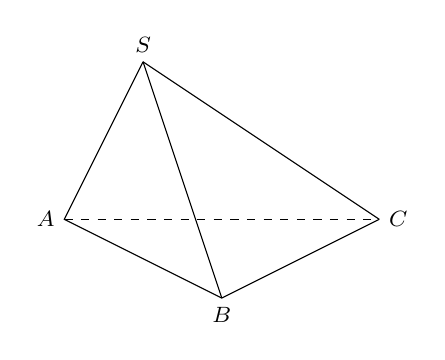
\begin{tikzpicture}
					\draw
					(0,0) coordinate [label=left:$A$] (A)
					(4,0) coordinate [label=right:$C$]  (C) --
					(2,-1) coordinate [label=below:$B$]  (B) -- (A) --
					(1,2) coordinate [label=above:$S$]  (S) edge (C)	 edge (B);
					\draw[dashed] (A) -- (C);
				\end{tikzpicture}
		\end{center}
		\fi


		\begin{parts}
			\part
			\exonly{
				Determinare l'area della base $ABC$.
				%	Déterminer l’aire de la base $ABC$ de cette pyramide.
			}
			\solonly{\SI{3.5}{\square\metre}}
			\part
			\exonly{
				Determinare il volume di questa piramide.
				%	Déterminer le volume de cette pyramide.
			}
			\solonly{\SI{1}{\cubic\metre}}
		\end{parts}
	\end{qblock}

	\begin{qblock}
		\question
		\exonly{
			I vertici di un cubo di lato \SI{10}{\centi\metre} vengono tagliati affinché le facce del cubo diventino degli ottagoni regolari.
		}

		\begin{parts}
			\part
			\exonly{
				Disegnare uno schizzo della situazione.
				%	Faire un croquis de la situation.
			}

			\ifprintanswers
				\begin{tikzpicture}[baseline={($(current bounding box.north)-(0,1.6ex)$)},scale=0.6]
					%\tikzstyle{isometric}=[x={(0.710cm,-0.410cm)},y={(0cm,0.820cm)},z={(-0.710cm,-0.410cm)}]
					\tikzset{every path/.style={isometric}}
					\tikzset{face/.style={fill=gray!20}}
					\pgfmathsetmacro{\cubex}{4}
					\pgfmathsetmacro{\cubey}{4}
					\pgfmathsetmacro{\cubez}{4}
					\pgfmathsetmacro{\ratio}{1/3}

					\coordinate (FTR) at (0,0,0);
					\coordinate (FTL) at (-\cubex,0,0);
					\coordinate (FBL) at (-\cubex,-\cubey,0);
					\coordinate (FBR) at (0,-\cubey,0);
					\coordinate (BTR) at (0,0,-\cubez);
					\coordinate (BBR) at (0,-\cubey,-\cubez);
					\coordinate (BTL) at (-\cubex,0,-\cubez);
					\coordinate (BBL) at (-\cubex,-\cubey,-\cubez);


					\draw[dotted] (FBL) -- (BBL);

					\shadedraw[face] ($(FTR)!\ratio!(FTL)$) -- ($(FTL)!\ratio!(FTR)$) -- ($(FTL)!\ratio!(FBL)$) -- ($(FBL)!\ratio!(FTL)$) --
					($(FBL)!\ratio!(FBR)$) -- ($(FBR)!\ratio!(FBL)$) --
					($(FBR)!\ratio!(FTR)$) -- ($(FTR)!\ratio!(FBR)$) --cycle;
					%top face
					\shadedraw[face] ($(FTR)!\ratio!(FTL)$) -- ($(FTR)!\ratio!(BTR)$) -- ($(BTR)!\ratio!(FTR)$) -- ($(BTR)!\ratio!(BTL)$) --
					($(BTR)!\ratio!(BTL)$) -- ($(BTL)!\ratio!(BTR)$) --
					($(BTL)!\ratio!(FTL)$) --  ($(FTL)!\ratio!(BTL)$)
					-- ($(FTL)!\ratio!(FTR)$) --cycle;
					%right face
					\shadedraw[face] ($(FTR)!\ratio!(BTR)$) -- ($(BTR)!\ratio!(FTR)$) -- ($(BTR)!\ratio!(BBR)$) -- ($(BBR)!\ratio!(BTR)$) --
					($(BBR)!\ratio!(FBR)$) -- ($(FBR)!\ratio!(BBR)$) --
					($(FBR)!\ratio!(FTR)$) --  ($(FTR)!\ratio!(FBR)$)
					-- ($(FTR)!\ratio!(FBR)$) -- cycle;

					%top right corner
					\shadedraw[face] ($(FTR)!\ratio!(BTR)$) -- ($(FTR)!\ratio!(FTL)$) -- ($(FTR)!\ratio!(FBR)$) --cycle;
					%top left corner
					\shadedraw[face] ($(FTL)!\ratio!(BTL)$) -- ($(FTL)!\ratio!(FTR)$) -- ($(FTL)!\ratio!(FBL)$) --cycle;

					%bottom right corner
					\shadedraw[face] ($(FBR)!\ratio!(FTR)$) -- ($(FBR)!\ratio!(FBL)$) -- ($(FBR)!\ratio!(BBR)$) --cycle;

					%top right corner
					\shadedraw[face] ($(BTR)!\ratio!(FTR)$) -- ($(BTR)!\ratio!(BTL)$) -- ($(BTR)!\ratio!(BBR)$) --cycle;
					%\fill[red] (0,0,0) circle (2pt);
					\draw[dotted] (FTR)  -- (FTL)  -- (FBL)  -- (FBR)  -- cycle;
					\draw[dotted] (FTR) -- (BTR)  -- (BTL)  -- (FTL) -- cycle;
					\draw[dotted] (FTR) -- (FBR) -- (BBR)  -- (BTR) -- cycle;
				\end{tikzpicture}
			\fi
			\part
			\exonly
			{
				Calcolare l'area esterna totale del solido ottenuto.
				%	Calculer l’aire extérieure totale du corps ainsi obtenu
			}
			\solonly{\SI{556.42}{\square\centi\metre}}
			\part
			\exonly{
				Calcolarne il volume.
				%	Calculer son volume.
			}
			\solonly{\SI{966}{\cubic\centi\metre}}
		\end{parts}
	\end{qblock}

	\begin{qblock}
		\question
		\exonly{
			Calcolare l'altezza della piramide retta a base rettangolare $ABCD$ il cui vertice é $S$.
			Le misure seguenti sono conosciute: $AB$=\SI{20}{\centi\metre}, $BC$=\SI{23}{\centi\metre} e $AS$=\SI{32}{\centi\metre}.
		}

		\ifprintanswers   \else
			
			\begin{center}
				\begin{tikzpicture}[scale=0.7]
					\coordinate[label=left:$A$] (A) at (0,0);
					\coordinate[label=right:$B$] (B) at (4,0);
					\coordinate[label=below:$C$] (C) at ($(B)+(35:3)$);
					\coordinate[label=below:$D$] (D) at ($(A)+(35:3)$);
					\draw (A)-- (B)--(C)--(D)-- cycle;
					\draw (3,5) coordinate [label=above:$S$]  (S)  edge (A) edge (D) edge (C)	 edge (B);
	
				\end{tikzpicture}
			\end{center}
		\fi
		\solonly{\SI{28.14}{\centi\metre}}
	\end{qblock}

	\begin{qblock}
		\question
		\exonly{
			Da uno degli spigoli di un cubo tagliamo un tetraedro i cui spigoli misurano  $AP=AQ=$\SI{3}{\centi\metre} e $AR=$\SI{4}{\centi\metre}.
		}

		
		\begin{center}
			\begin{tikzpicture}[baseline={($(current bounding box.north)-(0,1.6ex)$)}]
				%\tikzstyle{isometric}=[x={(0.710cm,-0.410cm)},y={(0cm,0.820cm)},z={(-0.710cm,-0.410cm)}]
				%\tikzset{every path/.style={isometric}}
				\tikzset{face/.style={fill=gray!20}}
				\pgfmathsetmacro{\cubex}{2}
				\pgfmathsetmacro{\cubey}{2}
				\pgfmathsetmacro{\cubez}{2}
				\pgfmathsetmacro{\ratio}{1/3}
	
				\coordinate (FTR) at (0,0,0);
				\coordinate[label=left:$A$] (FTL) at (-\cubex,0,0);
				\coordinate (FBL) at (-\cubex,-\cubey,0);
				\coordinate (FBR) at (0,-\cubey,0);
				\coordinate (BTR) at (0,0,-\cubez);
				\coordinate (BBR) at (0,-\cubey,-\cubez);
				\coordinate (BTL) at (-\cubex,0,-\cubez);
				\coordinate (BBL) at (-\cubex,-\cubey,-\cubez);
				\coordinate[label=left:$R$] (R) at ($(FTL)!0.6!(BTL)$);
				\coordinate[label=left:$Q$] (Q) at ($(FTL)!0.6!(FBL)$);
				\coordinate[label=right:$P$] (P) at ($(FTL)!0.6!(FTR)$);
	
				\draw[dotted] (FTR)  -- (FTL)  -- (FBL)  -- (FBR)  -- cycle;
				\draw[dotted] (FTR) -- (BTR)  -- (BTL)  -- (FTL) -- cycle;
				\draw[dotted] (FTR) -- (FBR) -- (BBR)  -- (BTR) -- cycle;
				\draw[very thick] (FTL) -- (R) -- (P) -- (Q) --cycle;
				\draw[very thick]  (FTL) -- (Q) -- (P);
				\draw[very thick, dashed]  (R) -- (Q);
			\end{tikzpicture}
		\end{center}

		\begin{parts}
			\part
			\exonly{
				Calcolare il volume del tetraedro.
				%Calculer le volume du tétraèdre.
			}
			\solonly{\SI{6}{\cubic\centi\metre}}

			\part
			\exonly{
				Calcolare l'altezza del tetraedro rispetto alla base $PQR$.
				%Calculer la hauteur du tétraèdre relative à la base $PQR$.
			}
			\solonly{\SI{1.9}{\centi\metre}}
		\end{parts}
	\end{qblock}

	\begin{qblock}
		\question
		\exonly{
			Un prisma a base quadrata di lato $b=\SI{2}{\centi\metre}$ é inscritto in una piramide regolare a base quadrata di lato $a=\SI{6}{\centi\metre}$ e altezza $h=\SI{10}{\centi\metre}$.

		}


		\begin{parts}
			\part
			\exonly{
				Eseguire uno schizzo della situazione.
				%Faire un croquis de la situation.
			}
			\ifprintanswers
				\begin{tikzpicture}[baseline={($(current bounding box.north)-(0,1.6ex)$)},scale=0.4]
					%\tikzstyle{isometric}=[x={(0.710cm,-0.410cm)},y={(0cm,0.820cm)},z={(-0.710cm,-0.410cm)}]
					%\tikzset{every path/.style={isometric}}
					\tikzset{face/.style={fill=gray!20}}
					\pgfmathsetmacro{\cubex}{4}
					\pgfmathsetmacro{\cubey}{4}
					\pgfmathsetmacro{\cubez}{4}
					\pgfmathsetmacro{\ratio}{1/2}
					\pgfmathsetmacro{\shift}{-3.5cm}

					\coordinate (S) at (0,7,0);
					\coordinate (FL) at (-\cubex,0,\cubez);
					\coordinate (FR) at (\cubex,0,\cubez);
					\coordinate (BR) at (\cubex,0,-\cubez);
					\coordinate (BL) at (-\cubex,0,-\cubez);
					\coordinate (PFTR) at ($(FR)!\ratio!(S)$);
					\coordinate (PFTL) at ($(FL)!\ratio!(S)$);
					\coordinate (PBTL) at ($(BL)!\ratio!(S)$);
					\coordinate (PBTR) at ($(BR)!\ratio!(S)$);
					\coordinate (PFBR) at ([yshift=\shift] PFTR);
					\coordinate (PFBL) at ([yshift=\shift] PFTL);
					\coordinate (PBBL) at ([yshift=\shift] PBTL);
					\coordinate (PBBR) at ([yshift=\shift] PBTR);


					\draw (FL) -- (FR) -- (BR);
					\draw[dotted] (BR) -- (BL) --(FL);
					\draw (S) edge (FR)  edge (FL) edge (BR);
					\draw[dotted] (S)  edge (BL) ;

					\draw[thick] (PFTL) -- (PFTR) -- (PBTR) --(PBTL) -- cycle;
					\draw[thick] (PFBR) -- (PFBL) -- (PBBL) -- (PBBR) -- cycle;
					\draw[thick] (PFTL) -- (PFBL) (PFTR) -- (PFBR) (PBTL) --(PBBL) (PBTR)--(PBBR);

				\end{tikzpicture}
			\fi
			\part
			\exonly{
				Calcolare il volume del prisma.
				%Calculer le volume du prisme.

			}
			\solonly{\SI{26.67}{\cubic\centi\metre}}
		\end{parts}
	\end{qblock}

	\begin{qblock}
		\question
		\exonly{
			I vertici di un tetraedro di lato \SI{12}{\centi\metre} vengono tagliati affinché le facce del tetraedro divengano degli esagoni regolari.

			Determinare il volume del solido ottenuto.
			%Déterminer le volume du corps ainsi obtenu.
		}
		\solonly{\SI{173.48}{\cubic\centi\metre}}

		
		\begin{center}
			\begin{tikzpicture}[scale=2]
				\tikzset{every path/.style={isometric}}
				\pgfmathsetmacro{\a}{2/ sqrt(3)}
				\pgfmathsetmacro{\b}{sqrt(3)/2}
				\pgfmathsetmacro{\h}{sqrt(23/4)}
				\pgfmathsetmacro{\ratio}{1/3}
				\pgfmathsetmacro{\Ratio}{2/3}
	
				\coordinate (A) at ( 0,0,\a);
				\coordinate (B) at ( 1,0,-\b);
				\coordinate (C) at ( -1,0,-\b);
				\coordinate (S) at ( 0,\h,0);
				\draw[dotted] (A)--(B);
	
				\draw[dotted] (C) edge (B) edge (A);
				\draw[dotted] (S) edge (A) edge (B);
				\draw [dotted]  (S) edge (C);
	
				\shadedraw[dashed] ($(A)!\Ratio!(S)$) -- ($(B)!\Ratio!(S)$) -- ($(C)!\Ratio!(S)$) -- cycle;
				\draw ($(A)!\Ratio!(S)$) -- ($(B)!\Ratio!(S)$) ;
	
				\shadedraw[dashed] ($(A)!\ratio!(S)$) -- ($(A)!\ratio!(B)$) -- ($(A)!\ratio!(C)$) --cycle;
				\draw ($(A)!\ratio!(S)$) -- ($(A)!\ratio!(B)$);
	
				\shadedraw[dashed] ($(B)!\ratio!(S)$) -- ($(B)!\ratio!(A)$) -- ($(B)!\ratio!(C)$) --cycle;
				\draw ($(B)!\ratio!(S)$) -- ($(B)!\ratio!(A)$);
	
				\draw[dashed] ($(C)!\ratio!(S)$) -- ($(C)!\ratio!(A)$) -- ($(C)!\ratio!(B)$) --cycle;
	
				\shade ($(A)!\Ratio!(S)$) -- ($(B)!\Ratio!(S)$) -- ($(B)!\ratio!(S)$) -- ($(B)!\ratio!(A)$)--($(B)!\Ratio!(A)$) -- ($(A)!\ratio!(S)$) --cycle;
	
			\end{tikzpicture}
		\end{center}
	\end{qblock}

\end{questions}

\subsection{Solidi di rotazione}
\begin{questions}

	\begin{qblock}
		\question
		\exonly{
			Il rapporto tra l'apotema e il diametro di un cono retto é di $\frac{5}{6}$ (vale a dire che $\frac{l}{d}=\frac{5}{6}$).\\
			Il volume del cono é di \SI{2.7}{\cubic\centi\metre}.\\
			Calcolare la superficie laterale del cono.\\
		}
		\solonly{\SI{8.13}{\square\centi\metre}}
	\end{qblock}


	\begin{qblock}
		\question
		\exonly{
			Pratichiamo un foro circolare di \SI{10}{\centi\metre}  di diametro in una placca metallica.

			Disponiamo nel foro una sfera di raggio $R>\SI{5}{\centi\metre} $ e constatiamo che la parte visibile della sfera ha un'altezza di \SI{13}{\centi\metre}.

		}

		\begin{parts}
			\part
			\exonly{
				Eseguire uno schizzo della situazione.

			}
			\ifprintanswers
				\begin{tikzpicture}[scale=0.5,baseline={($(current bounding box.north)-(0,1.6ex)$)}]
					\pgfmathsetmacro{\radius}{3}
					\pgfmathsetmacro{\planex}{5}
					\pgfmathsetmacro{\planez}{2.5}
					\pgfmathsetmacro{\ang}{30}
					\draw (-\planex,{-sin(\ang)*\radius},\planez) -- (-\planex,{-sin(\ang)*\radius},-\planez) -- (\planex,{-sin(\ang)*\radius},-\planez)--(\planex,{-sin(\ang)*\radius},\planez);
					\shadedraw[shading=ball,ball color=gray!10] (0,0) circle (\radius cm);
					\draw[very thick] (0,{-sin(\ang)*\radius}) ellipse ({cos(\ang)*\radius} and 0.5);
					\draw[very thick] (\planex,{-sin(\ang)*\radius},\planez) -- (-\planex,{-sin(\ang)*\radius},\planez) ;
					\draw [dashed] (-0.7*\planex,{-sin(\ang)*\radius}) |- (0,\radius);
					\draw[latex-latex] (-0.7*\planex,{-sin(\ang)*\radius}) -- node[left] {\SI{13}{\centi\metre}} ({$(-0.7*\planex,{-sin(\ang)*\radius})$} |- {$(0,\radius)$});

					\draw[dashed] ({cos(\ang)*\radius},{-sin(\ang)*\radius}) -- ({cos(\ang)*\radius},-4) -|  ({-cos(\ang)*\radius},{-sin(\ang)*\radius});
					\draw[latex-latex] ({cos(\ang)*\radius},-4) -- node[below] {\SI{10}{\centi\metre}}({-cos(\ang)*\radius},-4);
				\end{tikzpicture}

			\fi




			\part

			\exonly{
				Determinare il volume della sfera.

			}
			\sol{\SI{1.74}{\cubic\deci\metre}}
		\end{parts}
	\end{qblock}



	\begin{qblock}
		\question
		\exonly{
			Vogliamo costruire una boa avente la forma di un settore sferico in modo che la superficie della calotta sia identica alla superficie laterale del cono.

		}

		\begin{parts}
			\part

			\exonly{
				Calcolare il raggio $r$ della calotta e il volume $V$ del settore sferico se $R=\SI{70}{\centi\metre}$
			}
			\solonly{$r=\SI{56}{\centi\metre}$ , $h=\SI{28}{\centi\metre}$ e \\ $V=\SI{287351}{\cubic\centi\metre}$}
			\part
			\exonly{
				Calcolare il raggio $r$ della calotta e il volume $V$ del settore sferico in funzione del raggio $R$ della sfera da cui viene estratto.}
			\solonly{
				$r=\dfrac{4}{5}R$ e $V=\dfrac{4}{15}\pi R^3$
			}

		\end{parts}

		\ifprintanswers   \else
		\begin{center}
			\begin{tikzpicture}[baseline={($(current bounding box.north)-(0,1.6ex)$)},scale=0.6]
				\pgfmathsetmacro{\radius}{3}
				\pgfmathsetmacro{\planex}{5}
				\pgfmathsetmacro{\planez}{2.5}
				\pgfmathsetmacro{\ang}{30}
				\pgfmathsetmacro{\err}{0.1}
				\coordinate (O) at (0,0);
				\draw[] (O) circle (\radius cm);
				%manteau secteur spherique
				\shadedraw[gray!10, color=black] ({cos(\ang)*\radius-\err},{sin(\ang)*\radius-\err}) -- (O) node [below] {$O$} -- node[below] {$R$} ({-cos(\ang)*\radius+\err},{sin(\ang)*\radius-\err});
	
				\shadedraw[thick] ({cos(\ang)*\radius},{sin(\ang)*\radius}) arc (0:-180:{cos(\ang)*\radius} and 0.4) arc (180-\ang:\ang:\radius);
	
				\shadedraw[very thick] ({cos(\ang)*\radius},{sin(\ang)*\radius}) arc (\ang:180-\ang:\radius);
	
				\draw[dotted]  ({cos(\ang)*\radius},{sin(\ang)*\radius}) arc (0:180:{cos(\ang)*\radius} and 0.4);
	
				\draw[dashed] (0,{sin(\ang)*\radius} ) -- node [above] {$r$} ({cos(\ang)*\radius},{sin(\ang)*\radius});
				\draw [dashed] (0,\radius + 1) -- (0, -\radius -1);
			\end{tikzpicture}
		\end{center}
		\fi
	\end{qblock}


	\begin{qblock}
		\question
		\exonly{
			In una sfera di raggio $R=\SI{1}{\metre}$ é inscritto un cilindro la cui superficie laterale vale la metà della superficie della sfera.

			Calcolare il volume del cilindro.
		}

		\ifprintanswers   \else
		\begin{center}
			\begin{tikzpicture}[baseline={($(current bounding box.north)-(0,1.6ex)$)},scale=2]
				\pgfmathsetmacro{\Radius}{1}
				\pgfmathsetmacro{\radius}{1/sqrt(2)}
				\pgfmathsetmacro{\height}{sqrt(2) /2 }
	
				\coordinate (O) at (0,0);
				\shadedraw[shading=ball,ball color=gray!10] (O) circle (\Radius);
				\draw (0,\height  ) ellipse ({\radius}  and 0.1);
				\draw(0,-\height ) ellipse ({\radius}  and 0.1);
				\draw[dotted] (O) ellipse ({\Radius} and 0.1);
				\draw (-\radius, \height) -- (-\radius,- \height);
				\draw (\radius, \height) -- (\radius, -\height);
				\draw[dashed] (0,\height + 0.5) -- (0,-\height -0.5);
				\draw[thick] (O) -- node[above] {$R$} (\Radius,0);
				%manteau secteur spherique
			\end{tikzpicture}
		\end{center}

		\fi


		\solonly{$V=\SI{2.2}{\cubic\metre}$}
	\end{qblock}


	\begin{qblock}
		\question
		\exonly{
			Calcolare il volume di un cono retto di altezza $h=\SI{15}{\centi\metre}$ nel quale é inscritta una sfera di raggio $r=\SI{6}{\centi\metre}$.
		}
		\solonly{\SI{2827.4}{\cubic\centi\metre}}

		\ifprintanswers   \else
		\begin{center}
			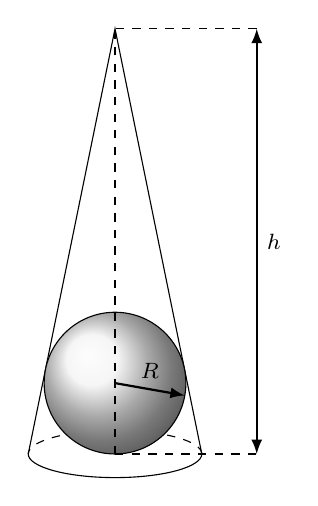
\begin{tikzpicture}[scale=0.3]
				\pgfmathsetmacro\radius{9/sqrt(6)}
				\coordinate (a) at (0,\radius);
				\coordinate (b) at (0,18);
				\draw (\radius,0) -- (b) -- (-\radius,0);
				\draw (\radius,0) arc(0:-180:{\radius} and 1);
				\draw[dashed] (\radius,0) arc(0:180:{\radius} and 1);
				%\fill[black] (0,0) circle (2pt) node[below left] { $O_1$};
	
	
				\shadedraw[shading=ball,ball color=gray!10] (0,3) circle (3);
				\draw[-latex,thick] (0,3) -- ++(-10:3) node[midway,above] {$R$};
	
				\draw[dashed] (0,0) -- (0,18);
				\draw[dashed] (0,0) -- (6,0)  (6,18) --(0,18);
				\draw[latex-latex,thick] (6,18) -- (6,0) node[midway, right] {$h$};
			\end{tikzpicture}
		\end{center}
		\fi
	\end{qblock}


	\begin{qblock}
		\question
		\exonly{
			Una sfera di raggio $R$  é illuminata da una sorgente luminosa puntiforme situata ad una distanza $L$ dal centro $O$ della sfera.
		}

		\begin{parts}
			\part

			\exonly{
				Calcolare la porzione (in \%) di superficie non illuminata della sfera se
				$R=\SI{1}{\metre}$ e $L=\SI{2.5}{\metre}$}
			\solonly{$70\%$}

			\part
			\exonly{
				Calcolare la proporzione si superficie non illuminata della sfera in funzione di $R$ e $L$.}

			\solonly{$\dfrac{(L+R)}{2L}$}
			\part
			\exonly{
				Discutere i due casi estremi $L \gg R$ (che potrebbe modellizzare la situazione Terra-Sole) e $L\approx R$.}
			\solonly{$50\%$ e $0\%$}

		\end{parts}



		\ifprintanswers   \else
			
			\begin{center}
				\begin{tikzpicture}
					\node[circle, draw, very thick] (c) at (0, 0) [minimum size=3cm] {};
					\fill[red]   (4, 0) coordinate (a) circle (3pt);
					\draw (tangent cs:node=c, point={(a)}, solution=1) coordinate (t1)-- (a);
					\draw (tangent cs:node=c, point={(a)}, solution=2) coordinate (t2)-- (a);
					%\draw[dashed] (0,0) -- (t1);
					%\draw[dashed] (0,0) -- (t2);
					\fill[gray!10] (t1)  let \p1 = ($ (0,0) - (t1) $) in  arc ({atan(\y1/\x1)}:{360-atan(\y1/\x1)}:1.5);
	
	
					\path ($(t1)!0.5!(t2)$) coordinate (e1);
	
					\fill[gray!10] (e1)  let \p1 = ($ (t2) - (t1) $) in  ellipse (0.2 cm and {0.5*veclen(\x1,\y1)});
					\node[circle, draw, very thick] (c) at (0, 0) [minimum size=3cm] {};
					\draw (t1) let \p1 = ($ (t1) - (t2) $) in
					arc (90:-90: 0.2 cm and {0.5*veclen(\x1,\y1)});
					\draw (0,0) -- node[below left] {$R$} (150:1.5);
					\fill (0,0) circle (1pt) node [below] {$O$};
					\draw [dashed] (0,0) -- (0,-2) -| (a);
					\draw [latex-latex] (0,-2) -- node [above] {$L$}({$(0,-2)$} -| {$(a)$});
	
				\end{tikzpicture}
			\end{center}
		\fi

	\end{qblock}


\end{questions}






\end{document}